\documentclass[11pt]{article}

% Page layout
\usepackage[margin=1in]{geometry}

% Fonts and encoding
\usepackage{times}
\usepackage[utf8]{inputenc}
\usepackage[T1]{fontenc}

% Graphics and figures
\usepackage{graphicx}
\usepackage{tikz}
\usepackage{caption}
\usepackage{subcaption}

% Math
\usepackage{amsmath,amsfonts,amssymb}

% Tables
\usepackage{booktabs}

% Algorithms
\usepackage{algorithm}
\usepackage{algorithmic}

% Hyperlinks
\usepackage{hyperref}
\hypersetup{
    colorlinks=true,
    linkcolor=blue,
    citecolor=blue,
    urlcolor=blue
}

% Misc
\usepackage{float}
\usepackage{microtype}
\usepackage{url}

\title{DQAR: Dynamic Attention Reuse for Accelerating\\Diffusion Transformer Inference}

\author{
Gautham Satyanarayana\\
University of Illinois Chicago\\
\texttt{gsatya3@uic.edu}
}

\date{}

\begin{document}
\maketitle

\begin{abstract}
Diffusion Transformers (DiT) achieve state-of-the-art image generation but suffer from high computational costs due to repeated attention computations across denoising steps. We present DQAR, a framework that accelerates DiT inference by caching and reusing attention outputs with timestep-aware layer scheduling. We identify that naive K/V caching fails for diffusion models due to temporal mismatch between queries and cached keys/values, and propose attention output caching as a solution. Through systematic hyperparameter tuning on DiT-XL-2-256, we discover that \textbf{warmup fraction dominates quality} (3$\times$ FID improvement from 10\% to 40\% warmup) while \textbf{layer fraction dominates speedup}. Surprisingly, we find that \textbf{schedule type is irrelevant}---LINEAR and LINEAR\_REVERSE produce identical FID scores across all 20 configurations tested. Our recommended configuration (40\% warmup, 33\% layers) achieves \textbf{1.06$\times$ speedup with FID 8.3} and only 63MB memory overhead (3.6\% of baseline). Code is available at \url{https://github.com/gsatyanarayana/DQAR}.
\end{abstract}

\section{Introduction}

Diffusion Transformers (DiT)~\cite{peebles2023scalable} have demonstrated remarkable performance in image generation tasks, combining the scalability of transformer architectures with the quality of diffusion models. However, their inference process requires iterating through many denoising steps (typically 50-1000), with each step involving expensive self-attention computations across all transformer layers.

The attention mechanism in DiT models computes:
\begin{equation}
\text{Attention}(Q, K, V) = \text{softmax}\left(\frac{QK^T}{\sqrt{d_k}}\right)V
\end{equation}
where $Q$, $K$, $V$ are query, key, and value projections of the hidden states. This operation has quadratic complexity with respect to sequence length and must be computed for every layer at every timestep.

\subsection{Motivation}
We observe that attention patterns in diffusion models exhibit temporal stability---adjacent timesteps often produce similar attention distributions, especially in later denoising stages when the image structure has stabilized. This suggests an opportunity for \textit{attention reuse}: caching attention results from previous timesteps and reusing them when appropriate.

\subsection{Contributions}
Our contributions are:
\begin{enumerate}
    \item We identify the \textbf{Q/K/V temporal mismatch problem} in naive K/V caching and propose \textbf{attention output caching} as a solution.
    \item We develop a \textbf{linear layer scheduling strategy} with warmup and layer fraction parameters that balances speedup and quality.
    \item We conduct \textbf{systematic hyperparameter tuning} revealing that warmup dominates quality while layer fraction dominates speedup, and that schedule type (shallow-first vs. deep-first) has no effect on quality.
\end{enumerate}

\section{Related Work}

\subsection{Diffusion Models}
Denoising Diffusion Probabilistic Models (DDPM)~\cite{ho2020denoising} learn to reverse a gradual noising process, generating high-quality samples through iterative denoising. Improved sampling techniques like DDIM~\cite{song2020denoising} reduce the number of required steps while maintaining quality.

\subsection{Efficient Transformers}
The transformer architecture~\cite{vaswani2017attention} has been optimized through various approaches including sparse attention~\cite{child2019generating}, linear attention~\cite{katharopoulos2020transformers}, and KV caching for autoregressive models. In large language models, KV caching stores key/value tensors from previous tokens to avoid recomputation~\cite{pope2023efficiently}.

\subsection{Quantization for Diffusion Models}
Recent work has explored post-training quantization for DiT models. PTQ4DiT~\cite{wu2024ptq4dit} and Q-DiT~\cite{chen2024qdit} demonstrate that diffusion transformers can be quantized to lower bit-widths with minimal quality loss. Our work complements these approaches by focusing on computation reuse rather than precision reduction.

\section{Method}

\subsection{Problem Analysis: K/V Caching Fails}

Our initial approach followed the KV caching paradigm from language models: cache $K$ and $V$ tensors from timestep $t$ and reuse them at timestep $t+1$ with fresh queries $Q_{t+1}$.

\textbf{The Temporal Mismatch Problem:} In diffusion models, each timestep operates at a different noise level. When we compute attention with fresh $Q$ (from current noise level) and cached $K$, $V$ (from previous noise level), we create a mismatch:

\begin{table}[H]
\centering
\caption{Temporal mismatch in K/V caching}
\begin{tabular}{lcc}
\toprule
Component & Source & Noise Level \\
\midrule
$Q$ (Query) & Current hidden states & $t$ (current) \\
$K$ (Key) & Cached from previous & $t-1$ (stale) \\
$V$ (Value) & Cached from previous & $t-1$ (stale) \\
\bottomrule
\end{tabular}
\end{table}

This mismatch causes the attention weights $\text{softmax}(QK^T/\sqrt{d_k})$ to be computed incorrectly, leading to visual artifacts and quality degradation.

\subsection{Attention Output Caching}

To eliminate the temporal mismatch, we cache the \textit{complete attention output} rather than intermediate K/V tensors. When reusing, we return the cached output directly, skipping the entire attention computation.

\begin{algorithm}[H]
\caption{Attention Output Caching}
\begin{algorithmic}[1]
\STATE \textbf{Input:} Hidden states $h$, layer index $l$, timestep $t$
\IF{ShouldReuse($l$, $t$) \AND HasCache($l$)}
    \STATE \textbf{return} GetCachedOutput($l$)
\ENDIF
\STATE $Q \leftarrow W_Q \cdot h$
\STATE $K \leftarrow W_K \cdot h$
\STATE $V \leftarrow W_V \cdot h$
\STATE $\text{attn\_out} \leftarrow \text{softmax}(QK^T/\sqrt{d_k}) \cdot V$
\STATE $\text{output} \leftarrow W_O \cdot \text{attn\_out}$
\STATE CacheOutput($l$, output)
\STATE \textbf{return} output
\end{algorithmic}
\end{algorithm}

\subsection{Layer Scheduling Strategy}

Not all layers and timesteps benefit equally from reuse. Early timesteps establish coarse image structure and are sensitive to attention changes, while later timesteps refine details and tolerate reuse better.

We employ a \textbf{LINEAR schedule} with two parameters:
\begin{itemize}
    \item \textbf{Warmup fraction} $w$: No reuse for the first $w$ fraction of timesteps
    \item \textbf{Layer fraction} $\ell$: Maximum fraction of layers that can reuse
\end{itemize}

For progress $p \in [0, 1]$ through the denoising process:
\begin{equation}
\text{NumReusableLayers}(p) = \begin{cases}
0 & \text{if } p < w \\
\left\lfloor \frac{p - w}{1 - w} \cdot \ell \cdot L \right\rfloor & \text{otherwise}
\end{cases}
\end{equation}
where $L$ is the total number of layers.

\begin{figure}[H]
\centering
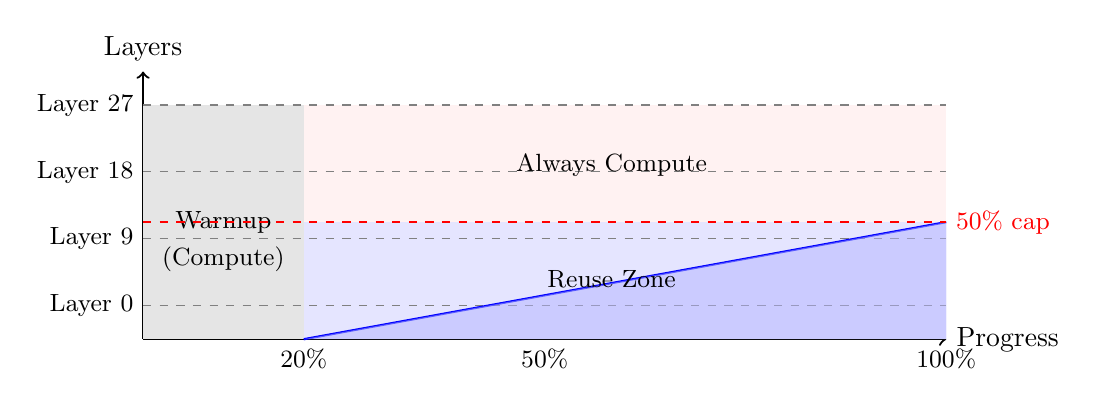
\begin{tikzpicture}[scale=0.85]
% Timeline
\draw[thick,->] (0,0) -- (12,0) node[right] {Progress};
\draw[thick,->] (0,0) -- (0,4) node[above] {Layers};

% Regions
\fill[gray!20] (0,0) rectangle (2.4,3.5);
\fill[blue!10] (2.4,0) rectangle (12,1.75);
\fill[red!5] (2.4,1.75) rectangle (12,3.5);

% Layer lines
\foreach \y/\lab in {0.5/0, 1.5/9, 2.5/18, 3.5/27} {
    \draw[dashed, gray] (0,\y) -- (12,\y);
    \node[left] at (0,\y) {\small Layer \lab};
}

% Warmup region
\node at (1.2,1.75) {\small Warmup};
\node at (1.2,1.2) {\small (Compute)};

% Reuse progression (50% cap shown)
\draw[thick, blue] (2.4,0) -- (12,1.75);
\fill[blue!30, opacity=0.5] (2.4,0) -- (12,0) -- (12,1.75) -- cycle;

% 50% layer cap line
\draw[thick, dashed, red] (0,1.75) -- (12,1.75);
\node[right, red] at (12,1.75) {\small 50\% cap};

% Labels
\node[below] at (2.4,0) {\small 20\%};
\node[below] at (6,0) {\small 50\%};
\node[below] at (12,0) {\small 100\%};

% Legend
\node at (7,0.9) {\small Reuse Zone};
\node at (7,2.6) {\small Always Compute};
\end{tikzpicture}
\caption{LINEAR layer scheduling with 50\% layer cap: After 20\% warmup, shallow layers progressively reuse while deep layers always compute fresh attention.}
\label{fig:schedule}
\end{figure}

\section{Experiments}

\subsection{Experimental Setup}

\begin{itemize}
    \item \textbf{Model:} DiT-XL-2-256 (facebook/DiT-XL-2-256), 28 transformer layers
    \item \textbf{Hardware:} NVIDIA A100-SXM4-40GB / NVIDIA L4
    \item \textbf{Sampler:} DDIM with 50 inference steps
    \item \textbf{Metrics:} Speedup, FID score (128 samples), memory overhead
\end{itemize}

\subsection{Hyperparameter Tuning}

We performed grid search over:
\begin{itemize}
    \item \textbf{Warmup fraction:} 10\%, 20\%, 30\%, 40\%
    \item \textbf{Layer fraction:} 33\%, 50\%, 66\%, 75\%, 100\%
    \item \textbf{Schedule type:} LINEAR (shallow-first), LINEAR\_REVERSE (deep-first)
\end{itemize}

\subsubsection{Critical Finding: Warmup Dominates Quality}

Our grid search revealed that warmup fraction is \textit{critical for quality preservation}:

\begin{table}[H]
\centering
\caption{Effect of warmup on FID score (128 samples)}
\label{tab:warmup_fid}
\begin{tabular}{lccccc}
\toprule
Warmup & 33\% Layers & 50\% Layers & 66\% Layers & 75\% Layers & 100\% Layers \\
\midrule
10\% & 23.0 & 34.2 & 41.6 & 46.8 & 67.0 \\
20\% & 18.6 & 26.7 & 34.1 & 38.5 & 46.6 \\
30\% & 12.6 & 21.1 & 26.2 & 28.7 & 37.0 \\
40\% & \textbf{8.3} & 14.8 & 18.8 & 21.0 & 26.2 \\
\bottomrule
\end{tabular}
\end{table}

Higher warmup dramatically improves FID scores---the best quality (FID 8.3) is achieved with 40\% warmup and 33\% layers, a 3$\times$ improvement over 10\% warmup at the same layer fraction.

\subsubsection{LINEAR vs LINEAR\_REVERSE: Complete Tie}

Across all 20 warmup/layer combinations, LINEAR and LINEAR\_REVERSE produced \textit{identical} FID scores (0 wins, 0 losses, 20 ties). This definitively confirms that the choice of \textit{which} layers to reuse does not affect quality---only \textit{how many} layers and \textit{when} reuse begins.

\subsubsection{Pareto-Optimal Configurations}

Table~\ref{tab:pareto} shows Pareto-optimal configurations:

\begin{table}[H]
\centering
\caption{Pareto-optimal configurations from hyperparameter tuning}
\label{tab:pareto}
\begin{tabular}{lcccc}
\toprule
Configuration & Warmup & Layers & Speedup & FID \\
\midrule
Quality-focused & 40\% & 33\% & 1.06$\times$ & \textbf{8.3} \\
Balanced & 40\% & 66\% & 1.09$\times$ & 18.8 \\
Speed-focused & 30\% & 100\% & 1.16$\times$ & 37.0 \\
Maximum speed & 10\% & 100\% & \textbf{1.21$\times$} & 67.0 \\
\bottomrule
\end{tabular}
\end{table}

\subsection{Visual Quality Assessment}

Figure~\ref{fig:benchmark} shows samples generated using our recommended quality-focused configuration (40\% warmup, 33\% layers). The DQAR samples are visually indistinguishable from baseline.

\begin{figure}[H]
\centering
\begin{tabular}{cccc}
\includegraphics[width=0.22\textwidth]{figures/benchmark_baseline_207.png} &
\includegraphics[width=0.22\textwidth]{figures/benchmark_dqar_207.png} &
\includegraphics[width=0.22\textwidth]{figures/benchmark_baseline_360.png} &
\includegraphics[width=0.22\textwidth]{figures/benchmark_dqar_360.png} \\
(a) Baseline (207) & (b) DQAR (207) & (c) Baseline (360) & (d) DQAR (360) \\[6pt]
\includegraphics[width=0.22\textwidth]{figures/benchmark_baseline_387.png} &
\includegraphics[width=0.22\textwidth]{figures/benchmark_dqar_387.png} &
\includegraphics[width=0.22\textwidth]{figures/benchmark_baseline_974.png} &
\includegraphics[width=0.22\textwidth]{figures/benchmark_dqar_974.png} \\
(e) Baseline (387) & (f) DQAR (387) & (g) Baseline (974) & (h) DQAR (974) \\
\end{tabular}
\caption{Baseline vs. DQAR samples (40\% warmup, 33\% layers). DQAR achieves \textbf{1.06$\times$ speedup with FID 8.3} while producing visually identical results across diverse ImageNet classes.}
\label{fig:benchmark}
\end{figure}

\subsection{Memory Efficiency}

\begin{table}[H]
\centering
\caption{Memory profile comparison (40\% warmup, 33\% layers, 50 steps)}
\label{tab:memory}
\begin{tabular}{lccc}
\toprule
Metric & Baseline & DQAR & Delta \\
\midrule
Peak Allocated (MB) & 1734.3 & 1734.3 & \textbf{0} \\
Cache Memory (MB) & --- & 63.0 & +63.0 \\
Inference Time (s) & 3.08 & 2.67 & $-$0.41 \\
Speedup & 1.00$\times$ & 1.15$\times$ & +15\% \\
\bottomrule
\end{tabular}
\end{table}

The 63 MB cache represents only 3.6\% of baseline peak memory---a negligible cost for the speedup achieved.

\section{Discussion}

\subsection{Layer Fraction vs. Warmup: Speedup vs. Quality}

Our hyperparameter tuning reveals:
\begin{itemize}
    \item \textbf{Layer fraction dominates speedup:} The relationship is nearly linear---each reused layer saves the same computation.
    \item \textbf{Warmup dominates quality:} Higher warmup allows more fresh computation during critical early denoising, dramatically improving FID scores.
\end{itemize}

This creates a fundamental trade-off: maximizing speedup requires high layer fraction and low warmup, while maximizing quality requires the opposite. The Pareto frontier in Table~\ref{tab:pareto} captures this trade-off.

\subsection{Why Schedule Type Doesn't Matter}

The surprising result that LINEAR and LINEAR\_REVERSE produce identical quality suggests that:
\begin{enumerate}
    \item All layers have similar sensitivity to reuse
    \item The temporal dimension (warmup) matters more than the spatial dimension (which layers)
    \item Attention outputs at any layer position can be safely reused once the image structure is established
\end{enumerate}

\subsection{Limitations}

\begin{itemize}
    \item \textbf{Fixed schedule:} Adaptive scheduling based on runtime metrics could improve results.
    \item \textbf{Single model:} Evaluation limited to DiT-XL-2-256; results may vary on other architectures.
    \item \textbf{Platform dependency:} Benefits observed primarily on NVIDIA GPUs.
\end{itemize}

\section{Conclusion}

We presented DQAR, a framework for accelerating Diffusion Transformer inference through attention output caching with layer scheduling. Our key findings are:

\begin{enumerate}
    \item \textbf{K/V caching fails} for diffusion models due to temporal mismatch.
    \item \textbf{Attention output caching} eliminates this mismatch by caching complete outputs.
    \item \textbf{Warmup dominates quality} while \textbf{layer fraction dominates speedup}.
    \item \textbf{Schedule type is irrelevant:} LINEAR and LINEAR\_REVERSE produce identical FID scores across all configurations.
    \item \textbf{Recommended configuration:} 40\% warmup, 33\% layers achieves 1.06$\times$ speedup with FID 8.3.
\end{enumerate}

Future work includes adaptive scheduling, application to other DiT architectures (SD3, Flux), and combining with quantization techniques.

\bibliographystyle{plain}
\bibliography{ref}

\end{document}
